\documentclass{standalone}

% graphics
\usepackage{tikz}
\usepackage{pgfplots}
\usepackage{siunitx}

\begin{document}

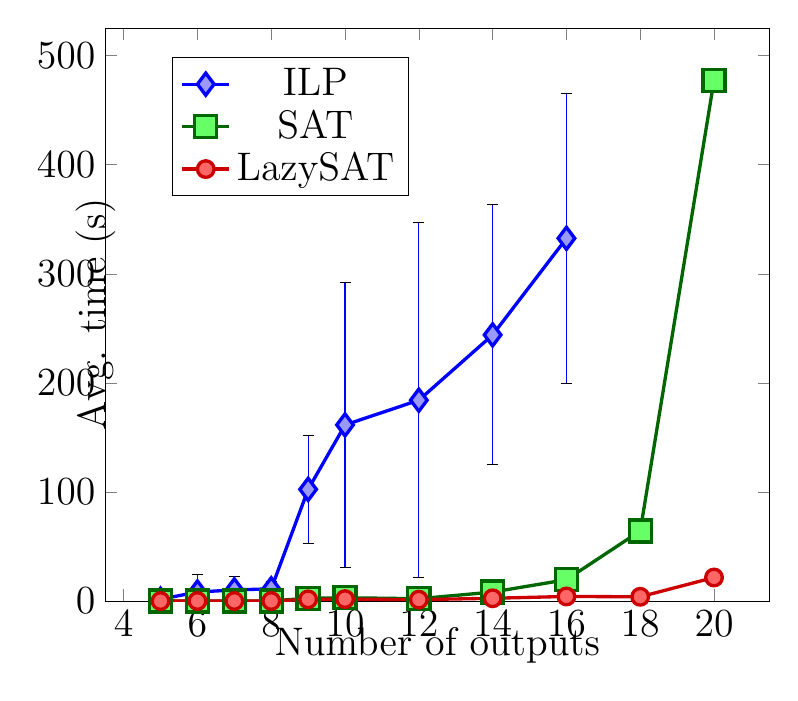
\begin{tikzpicture}[scale=1]
  \pgfplotsset{
      scale only axis,
      every x tick label/.append style={font=\Large},
      every y tick label/.append style={font=\Large},
	legend style={at={(0.1,0.95)},anchor=north west}
  }

\begin{axis}[
    legend style={font=\Large},
	xlabel={\Large Number of outputs},
	x label style={at={(axis description cs:0.5,-0.03)},anchor=north},
	y label style={at={(axis description cs:0.030,0.5)}, anchor=south},
	ylabel={\Large Avg. time (\si{\second})},
	ymin=0
]

% MIP
% dashdotdotted,
\addplot[mark=diamond*,  very thick, mark options={solid, fill=blue!40, mark size=4 pt}, draw=blue, error bars/.cd, y dir=both, y explicit] table [x=a, y=b, y error=c] {
a	b   c
5 	 1.689591932296753 	 0.49190848198898773
6 	 8.278921294212342 	 15.919799534395588
7 	 10.242094111442565 	 11.980815267206536
8    11.24408860206604 	 6.9857507776035
9 	 102.41729548999241 	 49.78164383418377
10 	 161.49013233184814 	 130.55777046716156
12 	 184.16992995738983 	 162.90848717783282
14 	 244.02930970191954 	 119.15690228480358
16 	 332.5471779505412 	 132.8263073188368
};
\label{LIP}
%18 	 521.7655539512634 	 0.0

%SAT
% error bars/.cd, y dir=both, y explicit,
\addplot[mark=square*, very thick, mark options={solid, fill=green!60, mark size=4 pt}, draw=black!60!green] table [x=a, y=b] {
a	b   c
5 	 0.06066195964813233 	 0.00263271158031934
6 	 0.11165335178375244 	 0.0828835845250046
7 	 0.14280121326446532 	 0.08669784316234681
8    0.14467639923095704 	 0.06363085747653752
9 	 2.61633677482605 	 1.9407879942235637
10 	 3.0609768629074097 	 2.144375166517033
12 	 2.198519062995911 	 1.1959526001500493
14 	 8.285453510284423 	 2.070259556891956
16 	 19.62026882171631 	 17.57617908955395
18 	 64.31706357002258 	 23.03657712317955
20 	 477.4083067689623 	 76.14931588615234
};
\label{SAT}  %SAT

%densely dashed, 
\addplot[mark=*, very thick, mark options={solid, fill=red!60, mark size=3pt}, draw=black!20!red, error bars/.cd, y dir=both, y explicit] table [x=a, y=b, y error=c] {
a   b   c
5 	 0.039904117584228516 	 0.0034616601208091527
6 	 0.067887282371521 	 0.05784900873241692
7 	 0.08147225379943848 	 0.05097189038492489
8    0.07803258895874024 	 0.037427662744407446
9 	 1.616580104827881 	 1.415788292961669
10 	 1.8442405939102173 	 1.2898197669496552
12 	 1.330327820777893 0.8304452495419578
14 	 2.5811299800872805 0.15116524890575167
16 	 4.2520509481430055 3.336145535787212
18 	 3.944814991950989 0.3824998939076343
20 	 21.631967997550966 6.581302712852444
};
\label{LazySAT}

\addlegendimage{/pgfplots/refstyle=LIP}
\addlegendentry{ILP}

\addlegendimage{/pgfplots/refstyle=SAT}
\addlegendentry{SAT}

\addlegendimage{/pgfplots/refstyle=LazySAT}
\addlegendentry{LazySAT}




\end{axis}
\end{tikzpicture}

\end{document}

